\documentclass[a4paper,10pt]{article}

\usepackage[utf8]{inputenc}
\usepackage[english]{babel}
\usepackage{algorithmicx}
\usepackage{algpseudocode}
\usepackage{amsmath}
\usepackage{dutchcal}
\usepackage{graphicx}
\usepackage{hyperref}
\usepackage{natbib}

\title{Enhanced and Extended Suffix Arrays}
\author{Adrian Regenfuß}

\begin{document}

\maketitle

\begin{abstract}
In this report, I review the literature on enhanced and extended suffix arrays
in the context of matching long strings. I examine the different algorithms
used for both constructing enhanced and extended suffix arrays and for using
them in searching long strings.
In the end, I compare enhanced and extended suffix arrays with suffix arrays
and suffix trees.
\end{abstract}

\section*{Introduction}

Finding the occurences of one string in another string, longest repeated
substrings and longest shared substrings of two different strings are
fundamental problems for many kinds of computing systems.

As a result, many different algorithms have been developed for these kinds
of problems: For finding the occurences of one string in another one the
naive algorithm and the Boyer-Moore algorithm (\citealt{boyer1977fast}),
and for all three of these problems (and more) three different data
structures: the suffix tree (\citealt{weiner1973linear}), the suffix
array (\citealt{manber1993suffix}) and the enhanced suffix array
(\citealt{abouelhoda2002enhanced}).

Suffix trees, suffix arrays and enhanced suffix arrays have the
disadvantage of requiring to be constructed for a specific string,
which has time and space requirements. Because of this, they are better
suited for tasks where immutable strings have to be searched or matched
repeatedly, although there has been some work to extend the suffix array
to dynamic strings (\citealt{salson2010dynamic}).

Since searching and matching very long immutable strings is very common
in genome analysis, it doesn't surprise that both suffix arrays and
enhanced suffix arrays were developed in that context.

This report first describes the enhanced suffix array as a data structure,
then sketches the algorithms used for constructing it, and afterwards
describes different string matching problems and how they are solved
by enhanced and extended suffix arrays. Finally, it compares enhanced
suffix arrays to normal suffix arrays and suffix trees, and closes with
an overview of tools that implement enhanced and extended suffix arrays.

\section*{Enhanced and Extended Suffix Arrays}

Enhanced suffix arrays were first proposed in
\citealt{abouelhoda2002enhanced} as an improvement over normal suffix
arrays. An enhanced suffix array contains a suffix array together with the
LCP-array of the string, and sometimes a Burrows-Wheeler transformation
and an inverse of the suffix table.

The term "Extended Suffix Array" is rarely used in the literature (e.g. in
\citealt{salson2010dynamic}) and seems to refer to a datastructure
combining the LCP array with the suffix array of a string. Since algorithms
that work on extended suffix arrays also work on enhanced suffix arrays,
I will focus on enhanced suffix arrays in this review.

For the following, let $S$ be a finite string of length $n$ over the
finite alphabet $\Sigma$.

\subsection*{suftab}

The suffix array $\hbox{suftab}$ is an array of integers describing the
positions of of sorted suffixes of $S$ in $S$.

More formally, let $\hbox{Suf}_{S}$ be the set of suffixes of $S$. Let
then $\hbox{SortSuf}_{S}$ be the array of lexically sorted suffixes of
$S$. Then $\hbox{suftab}[i]=k$ if and only if $S[k..n]=\hbox{SortSuf}[i]$.

For a string $S$ with $n=|S|<2^{32}$, $\hbox{suftab}$ usually uses $4n$
bytes.

\subsection*{lcptab}

The LCP (longest common prefix) table describes the length of the longest
common prefix of two neighbouring entries in the array of sorted suffixes.

Formally, $\hbox{lcptab}[i]=k$ iff
$\hbox{SortSuf}[i][0..k]=\hbox{SortSuf}[i-1][0..k]$. The zeroth entry
in $\hbox{lcptab}$ is always $0$.

For a string $S$ with $n=|S|$, $\hbox{suftab}$ usually uses $n$
bytes, assuming that the length of longest common prefixes
of two suffixes are less than 255. If this is not the case,
\citealt[sec. 8.1]{abouelhoda2004replacing} describes some practical
workarounds based on a secondary array.

\subsection*{bwttab}

Informally, $\hbox{bwttab}$ contains the character before the suffix in
$\hbox{suftab}$. It is derived from the Burrows-Wheeler transformation
used in text compression.
By containing $\hbox{bwttab}$, the enhanced suffix array contains a
complete copy of the original string which can be reconstructed in
linear time.

Formally, $\hbox{bwttab}$ is defined as follows:

\begin{equation}
	\hbox{bwttab}[i]=
	\begin{cases}
		S[\hbox{suftab}[i]-1] & \text{if} \hbox{suftab}[i]>0 \\
		\bot & \text{otherwise}
	\end{cases}
\end{equation}

In theory, the size of $\hbox{bwttab}$ depends on the size of the alphabet
$\Sigma$, but usually it is assumed that $|\Sigma|=256$, one ASCII
character. The space requirement of $\hbox{bwttab}$ then is $|S|=n$ bytes.

\subsection*{suftab$^{-1}$}

$\hbox{suftab}^{-1}$ is the inverse of the suffix array:
$\hbox{suftab}^{-1}[\hbox{suftab}[q]]=q$, or, in other words, when
viewing $\hbox{suftab}$ and $\hbox{suftab}^{-1}$ as permutations,
then the concatenation $\hbox{suftab}^{-1} \circ \hbox{suftab}=S_{id}$
($S_{id}$ is the identity permutation, also denoted by $(1)$ or $()$).

$\hbox{suftab}^{-1}$ requires the same amount of space as $\hbox{suftab}$,
$4n$ bytes.

The inverse suffix array is used in the tandem repeat finding algorithm.

\subsection*{Space requirements}

The space requirement of an enhanced suffix array is $10n$ bytes, $4n$
for each the suffix array and the inverse, and $n$ for burrows-wheeler
transformation and the lcp array.

\subsection*{Example}

For example, let $S=\hbox{"cagccacat"}$. Then $\hbox{suftab}$,
$\hbox{lcptab}$, $\hbox{bwttab}$, $\hbox{suftab}^{-1}$ and
$\hbox{suftab}$ are the following:

\begin{center}
	\begin{tabular}{ | l | c | c | c | c | l | }
		\hline
		i & suftab & lcptab & bwttab & $\hbox{suftab}^{-1}$ & SortSuf \\ \hline
		0 & 5 & 0 & c & 4 & acat\$ \\ \hline
		1 & 1 & 1 & c & 1 & agccacat\$ \\ \hline
		2 & 7 & 1 & c & 7 & at\$ \\ \hline
		3 & 4 & 0 & c & 6 & cacat\$ \\ \hline
		4 & 0 & 2 & $\bot$ & 3 & cagccacat\$ \\ \hline
		5 & 6 & 2 & a & 0 & cat\$ \\ \hline
		6 & 3 & 1 & g & 5 & ccacat\$ \\ \hline
		7 & 2 & 0 & a & 2 & gccacat\$ \\ \hline
		8 & 8 & 0 & a & 8 & t\$ \\ \hline
		9 & 9 & 0 & t & 9 & \$ \\ \hline
	\end{tabular}
\end{center}

\subsection*{LCP-Interval Trees}

An LCP-Interval of value $\ell$ ($\ell-[i..j]$) is an interval $[i..j]$ ($i \le j$)
for which holds:

\begin{itemize}
\item $\hbox{lcptab}[i]<\ell$
\item $\hbox{lcptab}[j+1]<\ell$
\item $\exists k: i<k\le j \land \hbox{lcptab}[k]=\ell$
\item $\forall k: i<k\le j \Rightarrow \hbox{lcptab}[k] \ge \ell$
\end{itemize}

One can visualize the lengths of the longest common prefixes as a
landscape, and LCP-intervals being regions in that landscape that have
a minimum height $\ell$.

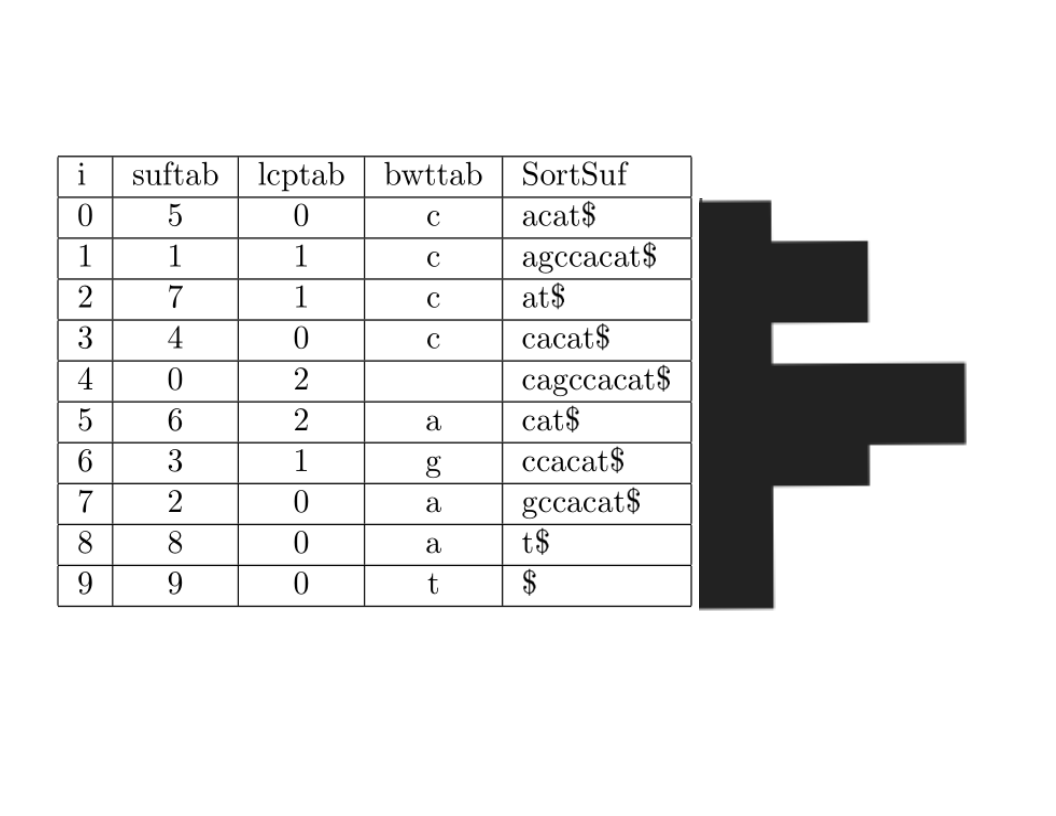
\includegraphics[width=\textwidth]{local_maxima.png}

LCP-intervals can be embedded into each other, specifically, an
$\mathcal{k}-[i..j]$ is embedded in $\mathcal{l}-[k..l]$ iff $k \le i
\le j \le l$ and $\mathcal{k}<\mathcal{l}$.

Due to this, the enhanced suffix array of a string implicitely contains
a data structure called the LCP-interval tree. The root of the tree
contains information on the 0-interval: $0-[0..n]$ with $n=|S|$. The
leaves are the 1-intervals, each containing the starting and ending
position of the corresponding LCP interval.

The LCP-interval tree is just the suffix tree (\citealt{weiner1973linear})
without leaves, and its traversal enables linear time solutions to some
string matching problems using the enhanced suffix array.

The LCP-interval tree is not saved in memory, but reconstructed
by using the suffix array and the LCP array during execution
(\citealt{abouelhoda2002enhanced}).

%Tree bottom-up traversal is from the root to the leaves,
%top-down is the other way around

\section*{Different String Matching Problems}

A plethora of different string matching problems have been identified
by computer scientists, for many of which suffix arrays and enhanced
suffix arrays are useful.

\citealt[pg. 2]{abouelhoda2004replacing} summarizes suffix tree applications
from \citealt[chap. 2]{gusfield1997algorithms} and classify them after their
type of tree traversal.

\subsection*{Exact String Matching}

\subsubsection*{Description}

Give a string $S$ of length $n$ and a string $T$ of length $m$ with $m
\le n$ both using them same alphabet $\Sigma$, the exact matches of $T$
in $S$ is the set of indices $I=\{i_1, \ldots, i_k\}$ for which holds
that $\forall i \in I: S[i..i+m]=T$.

In other words, $I$ is the set of indices where $T$ is a substring in $S$.

\subsubsection*{Suffix Array Algorithm}

\citealt{manber1993suffix} describes an exact string matching algorithm
that runs in ${\cal{O}}(m \log n)$ time and constant space.

Their proposed algorithm uses binary search to sequentially find
the first (smallest) index $L_{W}$ and the last (biggest) index
$R_{W}$ in $\hbox{suftab}$ so that $S[\hbox{suftab}[L_{W}]]$ and
$S[\hbox{suftab}[R_{W}]]$ have the prefix $T$.

First, it searches $L_{W}$ using binary search on the whole array
$\hbox{suftab}$ and then uses $L_{W}$ as a left boundary to find $R_{W}$,
again by binary search.  Using $L_{W}$ as a left boundary improves
runtime as opposed to two independent searches over the whole array,
although the latter might be easier to parallelize.

\subsubsection*{Extended Suffix Array Algorithm}

\citealt{manber1993suffix} then propose a speed improvement based on
longest common prefixes that reduces the runtime to ${\cal{O}}(m + \log
n)$. Their method attempts to reduce the number of single-character
comparisons by only comparing characters that occur after the longest
common prefix of $T$ and $S[M_{W}]$ ($M_{W}$ being the index in the
middle between $L_{W}$ and $R_{W}$).

\citealt[p. 152]{gusfield1997algorithms} describes another speed-up
called the super-accelerant, which uses LCP-arrays to in practice reduce
runtime even further. It doesn't improve worst-case time complexity.

%They then go on to explain a more complicated method,
%and Gusfield expands on their work on pg. 152 (84 in the PDF).

I have not come across a proposal to use interpolation search first
described in \citealt{perl1978interpolation} to search the suffix array
with an improved ${\cal{O}}(\log \log n)$ runtime. This perhaps stems
from the fact that interpolation search assumes uniform distribution of
the alphabet, and has a worst-case runtime of ${\cal{O}}(n)$. It still
might be useful to empirically test speed differences in binary and
interpolation search.

\subsection*{Supermaximal and Maximal Repeats}

Enhanced suffix arrays were first designed to solve problems
in genome analysis, especially finding segmental duplications
(\citealt{lander2001initial}). Due to this, many algorithms have been
devised for finding different kinds of repeated substrings in a string
$S$.

\subsubsection*{Description}

Two substrings $S_1=S[i_1..j_1]$ and $S_2=S[i_2..j_2]$ are called a
repeated pair if $S_1=S_2$ and $i_1 \ne i_2$ and $j_1 \ne j_2$.  $S_1$
and $S_2$ are furthermore a maximal repeat iff $S[i_1-1] \ne S[i_2-1]$
and $S[j_1+1] \ne S[j_2+1]$. A supermaximal repeat is a maximal repeat
that does not occur as a substring of another maximal repeat.

Let $S_a$ and $S_b$ be two distinct strings over $\Sigma$. Let $\#
\not \in \Sigma$ be a character. Then a maximum unique match (MUM) is
a supermaximal repeat $((i_a, j_a)(i_b, j_b))$ of $S_a\#S_b$ so that
$j_a<|S_b|$ and $i_b>|S_a|$.

For example, the string "xabyabwabyz" contains the maximal repeat "ab"
(at positions $((1,2),(4,5))$ and $((4,5)(7,8))$) and the maximal repeat
"aby" at positions $((1,3),(7,9))$, as well as the supermaximal repeat
"aby" as positions $((1,3),(7,9))$. Note that the set of supermaximal
repeats is a subset of the set of maximal repeats.

\subsubsection*{Enhanced Suffix Array Algorithm for Finding Supermaximal Repeats}

Finding supermaximal repeats using an enhanced suffix array is
comparatively simple; the process can be visualized as finding
local maxima in $\hbox{lcptab}$  with pairwise distinct values in
$\hbox{bwttab}$.

\begin{algorithmic}
\State $\hbox{maxstart} \gets 0$
\State $\hbox{result} \gets \emptyset$
\For {$i$ in $0..n-1$}
	\If {$\hbox{lcptab}[i]>\hbox{lcptab}[i-1] \hbox{ and } i>0$}
		\State $\hbox{maxstart} \gets i$
		\State $\hbox{supmaxrep} \gets true$
		\State $\hbox{preceding} \gets \emptyset$
	\ElsIf {$\hbox{lcptab}[i]<\hbox{lcptab}[i-1] \hbox{ and } \hbox{supmaxrep}$}
		\State $\omega \gets S[\hbox{suftab}[i-1]..\hbox{suftab}[i-1] +\hbox{lcptab}[i-1]]$
		\State $\hbox{result} \gets \hbox{result} \cup \{(\omega, \hbox{maxstart}, i-1)\}$
		\State $\hbox{supmaxrep} \gets false$
	\EndIf
	\If {$\hbox{bwttab}[i] \in \hbox{preceding}$}
		\State $\hbox{supmaxrep} \gets false$
	\Else
		\State $\hbox{preceding} \gets \hbox{preceding} \cup \hbox{bwttab}[i] $
	\EndIf
\EndFor
\end{algorithmic}

This algorithm runs in $\mathcal{O}(n)$ time and is described first by
\citealt{abouelhoda2002enhanced}.

\subsubsection*{Finding Maximum Unique Matches}

Finding MUMs is just a special case of finding supermaximal repeats:

\begin{itemize}
\item The enhanced suffix array of $S_a\#S_b$ is generated
\item The algorithm for finding supermaximal repeats is executed
\item The set of supermaximal repeats is scanned for instance where $j_a<|S_b|$ and $i_b>|S_a|$
\end{itemize}

This algorithm also runs in $\mathcal{O}(n)$ time ($n=|S_a\#S_b|$).

While this is theoretically good, in practice the construction
of the enhanced suffix array for the two strings provides
some hurdles. Especially in the case of sequence assembly
(\citealt{myers2000whole}), where the maximum unique matches of sometimes
tens of thousands of reads have to be assembled, re-constructing the
enhanced suffix arrray for each pair of reads can be computationally
quite intensive. \citealt{salson2010dynamic} describes techniques for
updating modified suffix arrays and LCP arrays, which could be a useful
starting point for finding methods of combining enhanced suffix arrays
of concatenated strings.

\subsubsection*{LCP-interval tree Traversal}

Since the LCP-interval tree is simply the suffix tree without leaves, it
is very useful to being able to construct and traverse the LCP-interval
tree using the enhanced suffix array.

\citealt{abouelhoda2002enhanced} expand on an algorithm proposed in
\citealt{kasai2001linear} that traverses the LCP-interval tree bottom
up and calls a function $process$ for each node in the tree.

The information passed to $process$ consists of a tuple $(\ell, lb, rb,
children)$, where $lb$ is the left boundary of the $\ell$-interval,
$rb$ is the right boundary, and $children$ is a list containing the
child intervals of the given $\ell$-interval (possibly being the empty
list $[]$).

The algorithm traverses the LCP-interval linearly and has two different
components:

\begin{itemize}
\item While the $\ell$-value of the interval on the top of the stack
is greater than $\hbox{lcptab}[i]$, pop the interval and process it,
then add it to the children of the new top of the stack
\item If the $\ell$-value of the interval on the top of the stack is
smaller than $\hbox{lcptab}[i]$, create a new interval at the top of
the stack ($lb=i, rb=\bot, children=[]$)
\end{itemize}

This algorithm runs in $\mathcal{O}(n)$ time.

\subsubsection*{Enhanced Suffix Array Algorithm for Finding Maximal Repeats}

One possible application of LCP-interval tree traversal is the detection
of maximal repeats in a string.

\citealt{abouelhoda2002enhanced} describe an algorithm that finds maximal
repeats in $\mathcal{O}(kn+z)$ time, where $k=|\Sigma|$ and z is the
amount of maximal repeats. For this, it uses lcp-interval tree traversal
to build position sets for an interval and its child interval and to
output position sets for distinct characters. It uses $\hbox{lcptab}$,
$\hbox{bwttab}$ and $\hbox{suftab}$.

A position set $\mathcal{P}_{[i..j]}(a)$ is the set of all positions in
an $\ell$-interval $[i..j]$ that are preceded by the character $a \in
\Sigma \cup \{\bot\}$:

$$\mathcal{P}(a)= \{ p \in \ell-[i..j] | \hbox{bwttab}[p]=a\}$$

This means that for a 1-interval $[i..i+1]$, $\mathcal{P}(a)$ is
$\emptyset$ for all a except $\hbox{bwttab}[i]$.

The current position set is saved on a per-function persistent stack. Let
$\mathcal{P}_{[i'..j']}(a)$ be the position set at the top of the stack
for $a \in \Sigma \cup \bot$ (position sets for all $a \in \Sigma \cup
\bot$ are saved on the stack).

Given the child position sets $\mathcal{P}_{[i'..j']}(a)$ and the current
position sets $\mathcal{P}^{q}_{[i..j]}(a)$ ($i<i'<j'<j$) for all $a
\in \Sigma \cup \bot$ ($[i..j]$ being an $\ell$-interval, $[i'..j']$
being an $\ell+1$-interval), output $(p, p+\ell-1), (p',p'+\ell-1))$ for
$p \in \mathcal{P}^{q}_{[i..j]}(a)$ and $p' \in \mathcal{P}^{q}_{[i..j]}(b)$
for $a, b \in \Sigma \cup \bot$, $a \not = b$.

The position sets are then combined and saved on the stack:
$\mathcal{P}^{q+1}_{[i..j]}(e):=\mathcal{P}^{q}_{[i..j]}(e) \cup
\mathcal{P}_{[i'..j']}(e)$ for all $e$ in the alphabet.

\section*{Construction}

\subsection*{Of the Suffix Array}

The naive construction of the suffix array (sorting the suffixes
lexically while saving their positions) uses $\mathcal{O}(n^2 \log n)$
time ($n^2 \log n$ instead of $n \log n$ because each suffix comparison
can at worst use $\mathcal{O}(n)$ time). If done in place (e.g. using
pointers), it uses $\mathcal{O}(n)$ space. \citealt{manber1993suffix} use
radix sort.

Several $\mathcal{O}(n)$ algorithms have been developed for sorting
suffixes: the skew algorithm described by \cite{karkkainen2003simple}
or the pure-induced sorting from \citealt{nong2009linear}.

\subsection*{Of the Inverse Suffix Array}

Neither \citealt{abouelhoda2004replacing} nor
\citealt{abouelhoda2002enhanced} describe an algorithm for constructing
inverse suffix arrays. Since the algorithm is quite straightforward,
it can be listed here:

\begin{algorithmic}
\For {$i$ in $0..n-1$}
	\State $\hbox{suftab}^{-1}[\hbox{suftab}[i]] \gets i$
\EndFor
\end{algorithmic}

This is a straightforward implementation of the definition of the inverse
suffix array, and the algorithm has time complexity $\mathcal{O}(n)$.

\subsection*{Of the LCP Array}

The LCP array can be constructed in linear time from the
suffix tree by first constructing the suffix tree in linear time
(\cite{giegerich1997ukkonen}), then removing the leaves to create the
LCP interval tree, and then traversing the LCP interval tree to generate
the LCP array. All steps run in $\mathcal{O}(n)$, so in combination they
also run in $\mathcal{O}(n)$.

Alternatively, one can use the induced sorting algorithm
(\cite{fischer2011inducing}) to compute both suffix arrays and LCP-arrays.

\subsection*{Of the Burrows-Wheeler Transform Array}

The BWT array can be constructed in linear time from the suffix array
using the naive algorithm (just linearly traversing the suffix array
and executing $\hbox{bwttab}[i]=S[\hbox{suftab}[i]-1]$).

\section*{Comparison}

The enhanced suffix array was developed as an alternative to the Suffix
Tree, which has been a successful and fast data structure in genome
analysis, but uses a lot of memory. Specifically, the suffix tree uses
about 20 bytes per input character (\cite{kurtz1999reducing}). The
goal was to create a datastructure with which one can solve the same
problems as the suffix tree, with the same time complexity, but which
uses less space.

The enhanced suffix array uses 10 bytes per input character under plausible
assumptions:

\begin{itemize}
\item $\hbox{suftab}$ uses $4n$ bytes (assuming $|S| \le 2^{32}$)
\item $\hbox{suftab}^{-1}$ uses $4n$ bytes as well
\item $\hbox{lcptab}$ uses $n$ bytes (usually assuming LCP values $<255$, although \citealt{abouelhoda2004replacing} describes how to use a secondary array to manage extreme cases)
\item $\hbox{bwttab}$ uses $n$ bytes (assuming $|\Sigma| \le 255$)
\end{itemize}

On disk, an enhanced suffix array then uses $10n$ bytes instead of
$20n$ bytes for a suffix tree, but most algorithms for Enhanced Suffix
Arrays don't use every component, but are usually restricted (e.g. exact
string matching only needing $\hbox{suftab}$ and $\hbox{lcptab}$, and
$\hbox{suftab}^{-1}$ only being required for finding tandem repeats).
This means that practical working memory requirements during runtime
are usually even smaller.

Enhanced suffix arrays also carry the benefit of a linear layout
in memory, which increases cache performance as compared to less
linear suffix trees, and often offer practical speedups to existing
implementations (see \citealt[sec. 7]{abouelhoda2002enhanced}).

\section*{Applications}

Enhanced suffix arrays have been used in bioinformatics
software such as \href{http://vmatch.de/}{VMatch}
(see \citealt{kurtz2003vmatch}), subsuming the
\href{https://bibiserv.cebitec.uni-bielefeld.de/reputer/}{REPuter project}
(see \citealt{kurtz2001reputer}).

However, many genome comparison software projects use
suffix trees instead of enhanced or extended suffix array,
such as \href{http://mummer.sourceforge.net/}{MUMmer}
(\citealt{kurtz2004versatile}).

\section*{Conclusion}

I have presented the enhanced suffix array and the algorithms it uses
to solve several string matching problems, among them finding maximal
and supermaximal repeats and exact string matching.
The enhanced suffix array presents a viable alternative to other string
matching datastructures such as the suffix tree: the construction
algorithms have a comparable time complexity ($\mathcal{O}(n)$), as well
as the the specific string matching problems ($\mathcal{O}(m + \log n)$
for exact string matching, $\mathcal{O}$ for finding supermaximal repeats
and MUMs, and $\mathcal{O}(|\Sigma|n+z)$ for finding maximal repeats).
Beyond that, in practice enhanced suffix arrays use less working memory
than suffix trees and often have faster execution times due to linear
layout in memory.

I have not covered algorithms for finding tandem repeats, methods for
updating enhanced suffix arrays when the underlying string $S$ changes,
and compressed enhanced suffix arrays.

\bibliographystyle{plainnat}
\bibliography{sources}

\end{document}
